
\documentclass[%
        %draft,
        %submission,
        %compressed,
        final,
        %
        %technote,
        %internal,
        %submitted,
        %inpress,
        %reprint,
        %
        %titlepage,
        notitlepage,
        %anonymous,
        narroweqnarray,
        inline,
        %twoside,
        ]{ieee}
%
% some standard modes are:
%
% \documentclass[draft,narroweqnarray,inline]{ieee}
% \documentclass[submission,anonymous,narroweqnarray,inline]{ieee}
% \documentclass[final,narroweqnarray,inline]{ieee}

\usepackage{ieeefig,url,enumerate}

\begin{document}

\title{Scaling Machine Learning Algorithms}

% format author this way for journal articles.
\author[SHORT NAMES]{
  Juan Batiz-Benet \\
  \and{\quad\quad}
  Quinn Slack \\
  \and{\quad\quad}
  Matt Sparks \\
  \and{\quad\quad}
  Ali Yahya
}

% specifiy the journal name
%\journal{IEEE Transactions on Something, 1997}

% Or, when the paper is a preprint, try this...
%\journal{IEEE Transactions on Something, 1997, TN\#9999.}

% Or, specify the conference place and date.
%\confplacedate{Ottawa, Canada, May 19--21, 1997}

\maketitle

\begin{abstract}
We wish to provide a portable framework for the rapid prototyping of machine
learning algorithms on a cluster of computers.
\end{abstract}

% do the keywords
%\begin{keywords}
%keyword 1, keyword 2 ...
%\end{keywords}

\section{Introduction}

% try out a theorem...
% \newtheorem{theorem}{Theorem}
% 
% \begin{theorem}[Theorem name]
%   Consider the system ...
% \end{theorem}
% 
% \begin{proof}
%   The proof is trivial.
% \end{proof}

\section{Distributing Work}

In order for an algorithm to be run in parallel on several machines, some part
of it must be amenable to parallelization. More specifically, some component or
step of the algorithm must be able to be subdivided into \emph{workunits} that
can be processed in parallel by multiple nodes with little or no communication
between the nodes. If communication between nodes is excessive, the overhead of
distributing the work becomes dominant and the any potential performance gained
by running in parallel is lost.

A significant fraction of learning algorithms work in an iterative manner and
depend on generic optimization routines like gradient descent, conjugate
gradient, or L-BFGS. Many of these routines are well suited for parallelization.
As an example, each iteration of batch gradient descent evaluates a function on
every input vector and then sums their results. Consequently, each iteration of
batch gradient descent can easily be parallelized by dividing the sum into $n$
disjoint partial sums, computing each partial sum on a separate slave machine,
and aggregating the results to compute the full sum.

\section{Rapid Prototyping}

Previous work has been done in distributing MATLAB. However, due to licensing
constraints, this is not feasible for large clusters. We needed to choose
another environment in which to develop and test machine learning
algorithms. For this project, we considered Python and R as alternatives to
MATLAB.

\subsection{Requirements}

At a high level, both 

Words here about why R and Python might be good choices. (Packages available
for matrix manipulations, highly general, free, easy to pick up and use,
portable?)


\subsection{Performance Benchmarks}

We benchmarked the performance of R against Python's (using the numpy package).
In order to avoid implementation or algorithm-specific bias, we decided to
benchmark common linear algebra functions (e.g. matrix multiplication)
ubiquitous in learning algorithms.

The following tables show the running times of python and R on various
operations using different matrix or vector sizes, as well as the time ratio of
python / R. Every test ran 10000 operations.

\begin{center}
  \vspace{1em}
    \textbf{Matrix Addition} \\
\begin{tabular}{cccc}
size  & python  &  R       & python / R \\
  \hline
50  & 0.0060 & 0.0159 & 0.3774 \\
75  & 0.0110 & 0.0302 & 0.3642 \\
100 & 0.0170 & 0.0519 & 0.3276 \\
150 & 0.0350 & 0.1161 & 0.3015 \\
250 & 0.0950 & 0.3396 & 0.2797 \\
\hline
\end{tabular}

\vspace{1em}
    \textbf{Matrix Multiplication} \\
\begin{tabular}{cccc}
size  & python  &  R       & python / R \\
  \hline
50  & 0.1600  & 0.2208  & 0.7246 \\
75  & 0.5800  & 0.7339  & 0.7903 \\
100 & 1.3030  & 1.6323  & 0.7983 \\
150 & 4.2350  & 5.2311  & 0.8096 \\
250 & 18.9190 & 22.9759 & 0.8234 \\
\end{tabular}

\vspace{1em}
    \textbf{Element-Wise Matrix Multiplication} \\
\begin{tabular}{cccc}
size  & python  &  R       & python / R \\
  \hline
150   & 0.0350  &  0.1576  &  0.2221 \\
225   & 0.0760  &  0.3741  &  0.2032 \\
300   & 0.1510  &  0.6859  &  0.2201 \\
450   & 0.9310  &  2.0938  &  0.4446 \\
750   & 3.3010  &  5.4117  &  0.6100 \\
\end{tabular}

\vspace{1em}
    \textbf{Matrix Transpose} \\
\begin{tabular}{cccc}
size  & python  &  R       & python / R \\
  \hline
50  & 0.0010  & 0.0325 & 0.0308 \\
75  & 0.0010  & 0.0610 & 0.0164 \\
100 & 0.0010  & 0.1030 & 0.0097 \\
150 & 0.0010  & 0.2196 & 0.0046 \\
250 & 0.0010  & 0.6119 & 0.0016 \\
\end{tabular}

\vspace{1em}
\textbf{Vector inner product} \\
\begin{tabular}{cccc}
size  & python  &  R       & python / R \\
  \hline
2500  & 0.0040 & 0.0523 & 0.0765 \\
3750  & 0.0060 & 0.0772 & 0.0777 \\
5000  & 0.0070 & 0.1030 & 0.0680 \\
7500  & 0.0100 & 0.1519 & 0.0658 \\
12500 & 0.0160 & 0.2514 & 0.0636 \\
\end{tabular}

\end{center}

In terms of performance, Python is the clear winner. It outperforms R in every
case, most of the cases by an order of magnitude. In the worst case, Python
takes 80\% of the time that R takes.

Perhaps also some words here about why Python is still acceptable even if it is
significantly slower than MATLAB. In particular, we are doing rapid
prototyping, so peak CPU performance isn't the deciding factor. We are more
interested in processing lots of data by distributing it to enough nodes such
that the data can fit in memory and be processed effectively.

\subsection{Style Benchmarks}

When prototyping algorithms, the clarity of a language plays a significant role.
MATLAB's simplicity and conciseness, yielding very clear and readable code, can
significantly reduce implementation bugs and ads minimal overhead to expressing
the algorithm in code. This is not the case for languages like C++, where
performance and reliability are more important than readability.

On one hand, R is stylistically very similar to MATLAB. Matrix and list
operations are just as straightforward, and it provides inbuilt equivalents of
most of MATLAB's probability and statistics packages. Further, the R interpreter
makes it just as easy as MATLAB to plot and visualize data structures.

On the other hand, Python's syntax is less suited for matrix operations.
However, Python's Numpy package includes Matlib, an interface that attempts to
emulate MATLAB's syntax. It is designed specifically for MATLAB programmers and
to ease the porting of MATLAB code. Certain syntactic elements are still overly
verbose (e.g. M.transpose() vs M') and may hinder the readability of any given
algorithm.

Strictly from a syntactic and stylistic perspective, R may be preferable to
Python because of its simplicity and closeness to MATLAB. However, because
of the results of the performance and functionality benchmarks presented above,
Python continues to be the best contender.

\section{Framework Design}

\subsection{Conventional Approaches}

Some words here about how the batch gradient descent example easily lends
itself to a straight mapreduce workflow. Because of this workflow, we first
considered using an existing mapreduce framework for our project.

One such framework we considered is Hadoop MapReduce. Some words here about why
Hadoop doesn't apply well to our problem. Consider the batch gradient decent
example again. Each iteration is essentially a mapreduce operation: the
examples are split up and distributed, the individual sums are calculated at
each node, and the reduce operation is calculating the final sum. The examples
considered at each node must remain stored locally at that node, ideally in
memory, for later recall during the next mapreduce operation for the subsequent
iteration.

Some words here about Disco and its attempt to solve this problem?

\subsection{Our design}

Our design consists of a single master and one or more slaves, as shown in
Fig. \ref{diagram}.

\begin{figure}[hb]
  \begin{center}
    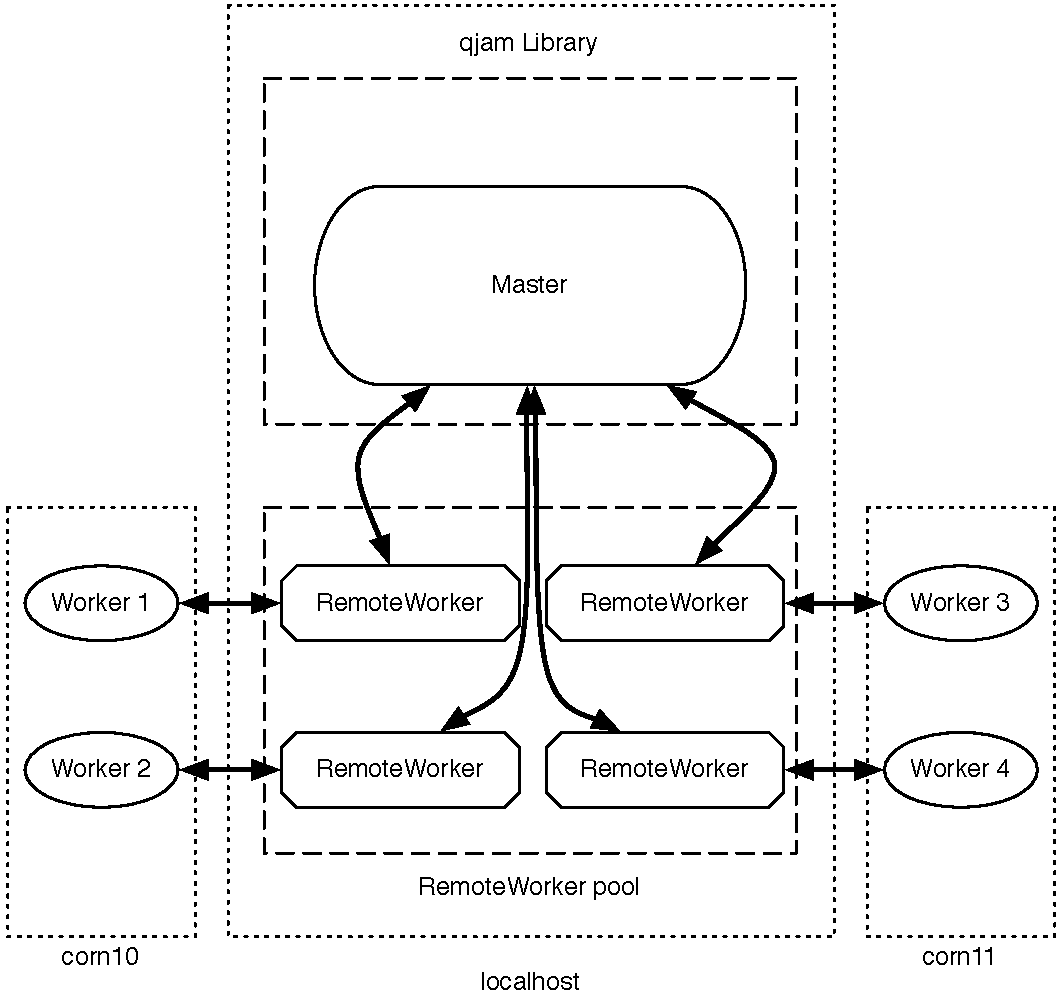
\includegraphics[width=2.5in]{fwk_diagram/fwk_diagram.pdf}
  \end{center}
  \caption{Diagram of our framework.}
  \label{diagram}
\end{figure}

First, on the master, you define a Python map function with the following prototype:
\begin{verbatim}
    def mymap(examples, params):
        psum = 0
        for (xi,yi) in examples:
            psum += (yi - g(params.theta.T * xi)) * xi
        return psum
\end{verbatim}

Then, also on the master, you specify your training examples and initial parameters:
\begin{verbatim}
    examples = ((x1, y1), (x2, y2), (x3, y3))
    params   = (0, 0, 0)
\end{verbatim}

The difference between examples and parameters is that examples will not be
resent on each iteration. We will check whether the slave already has the {\tt
  examples} object (with the same hash) and only resend it if needed. The
parameters data, however, will be resent for each iteration. These two objects
can be arbitrarily typed, as long as they are serializable. For example, for
large datasets, we might implement a list/dictionary proxy (that behaves like
its standard Python counterpart but doesn't store everything in memory). Also,
typically they will hold {\tt numpy} arrays and matrices instead of Python
tuples as shown in the example above.

To start the job, call:

\begin{verbatim}
    master.run(mymap, examples, params)
\end{verbatim}

This instructs the master to serialize the map function, training data, and
initial parameters, and send them to the slaves. Each slave will run the {\tt
  mymap} function, with the parameters in {\tt params} and some portion of the
training set available in {\tt examples}.

This call will block until all slaves respond with their partial sums. The {\tt
  run} method will apply the {\tt sum} reduce function to each slave's response
and will return the total sum. (For easy local testing, the {\tt mymap}
function can also be run on the local machine in the same Python process.)

We will initially ignore slave failures. Failure tolerance can be added
later (reship the local data, rerun dead slave's work). The master shares its fate
with the main program being run; if the main program dies, the master dies with
it, and vice versa. Thus, we do not need replicated masters or anything
similarly sophisticated.

\subsection{Serialization and Local Storage}

Some notes here about pickling functions and managing local storage at each
node.

The master divides the data and ships to each slave its share of the examples
(or whatever other data is needed).

% do the biliography:
%\bibliographystyle{IEEEbib}
%\bibliography{my-bibliography-file}

%----------------------------------------------------------------------
% FIGURES
%----------------------------------------------------------------------
% There are many ways to include figures in the text. We will assume
% that the figure is some sort of EPS file.
%
% The outdated packages epsfig and psfig allow you to insert figures
% like: \psfig{filename.eps} These should really be done now using the
% \includegraphics{filename.eps} command.
%
% i.e.,
%
% \includegraphics{file.eps}
%
% whenever you want to include the EPS file 'file.eps'. There are many
% options for the includegraphics command, and are outlined in the
% on-line documentation for the "graphics bundle". Using the options,
% you can specify the height, total height (height+depth), width, scale,
% angle, origin, bounding box "bb",view port, and can trim from around
% the sides of the figure. You can also force LaTeX to clip the EPS file
% to the bounding box in the file. I find that I often use the scale,
% trim and clip commands.
%
% \includegraphics[scale=0.6,trim=0 0 0 0,clip=]{file.eps}
%
% which magnifies the graphics by 0.6 (If I create a graphics for an
% overhead projector transparency, I find that a magnification of 0.6
% makes it look much better in a paper), trims 0 points off
% of the left, bottom, right and top, and clips the graphics. If the
% trim numbers are negative, space is added around the figure. This can
% be useful to help center the graphics, if the EPS file bounding box is
% not quite right.
%
% To center the graphics,
%
% \begin{center}
% \includegraphics...
% \end{center}
%
% I have not yet written good documentation for this, but another
% package which helps in figure management is the package ieeefig.sty,
% available at: http://www-isl.stanford.edu/people/glp/ieee.shtml
% Specify:
%
%\usepackage{ieeefig}
%
% in the preamble, and whenever you want a figure,
%
%\figdef{filename}
%
% where, filename.tex is a LaTeX file which defines what the figure is.
% It may be as simple as
%
% \inserteps{filename.eps}
%
% or
% \inserteps[includegraphics options]{filename.eps}
%
% or may be a very complicated LaTeX file.

\end{document}
